\documentclass[9pt]{beamer}
\mode<presentation>

% Theme choice:
\usetheme{Madrid}%Darmstadt 
\usepackage{xcolor}
\definecolor{mGreen}{rgb}{0,0.6,0}
\definecolor{mRed}{rgb}{0.6,0,0}
\usecolortheme[RGB={0,100,50}]{structure}
 \usefonttheme{structurebold} 
\setbeamercovered{invisible}
%\setbeamertemplate{navigation symbols}{}
\usepackage{dynblocks}
\usepackage{textpos}
\usepackage{amsfonts}
\usepackage{amsmath}
\usepackage{amssymb}
\usepackage{amsthm}
\usepackage{listings}
\usepackage{tikz}
\usepackage{pgfplots}
\pgfplotsset{compat=1.18}
\newtheorem{teorema}{Teorema}\usepackage{mathtools}
\renewcommand{\proofname}{Prova}
\usepackage[portuguese]{babel}

\uselanguage{Portuguese}
\languagepath{Portuguese}

\deftranslation[to=Portuguese]{Theorem}{Teorema}
\deftranslation[to=Portuguese]{Lemma}{Lema}
\deftranslation[to=Portuguese]{Corollary}{Corolário}
\deftranslation[to=Portuguese]{Proof}{Prova}

\usepackage{dutchcal}
\usepackage{hyperref}
\usepackage[utf8]{inputenc}
\usepackage[T1]{fontenc}
\usepackage{amsthm}


\usepackage[affil-it]{authblk} 
\usepackage{etoolbox}
\usepackage{lmodern}

\makeatletter
\patchcmd{\@maketitle}{\LARGE \@title}{\fontsize{18}{19.2}\selectfont\@title}{}{}
\makeatother

\renewcommand\Authfont{\fontsize{12}{14.4}\selectfont}
\renewcommand\Affilfont{\fontsize{9}{10.8}\itshape}

% Title page details: 
\title[Presentation]{ENGENHARIA DA QUALIDADE E CONFIABILIDADE} %add title


\institute[UniRV]{\textbf{\large  \textcolor{structure}{\textbf{\large
Arquiteturas tolerantes a defeitos: Sistemas de proteção, Arquitetura de automonitoramento, Programação N-versões (N-version programming) e Diversidade de software
}} %add name 
% \hspace{0.5pt}
\\ \qquad
\\Professor: Me. Sergio Souza Novak 
\\Faculdade de Engenharia de Software}
} 
% \titlegraphic{\includegraphics[width=5cm]{msu.eps}}
\titlegraphic{
\includegraphics[width=5cm]{Universidade_de_Rio_Verde.jpg}}
\date{}

% Logo only on title page
%\logo{
\includegraphics[width=1cm,keepaspectratio]{Logo.png}}
\usepackage[pscoord]{eso-pic}


\begin{document}

% Title page frame
%\begin{frame}
    %\titlepage 
%\end{frame}
\frame[plain]{\titlepage}
%logo
\AddToShipoutPictureFG{
    \put(\LenToUnit{.92\paperwidth},
    \LenToUnit{.185\paperheight})
    {\vtop{{\null}
    \makebox{
\includegraphics[width=.8cm,keepaspectratio]{Universidade_de_Rio_Verde.jpg}}}}}


\begin{frame}{Sumário}
  \tableofcontents
\end{frame}
\section{Arquiteturas Tolerantes a Defeitos}

\begin{frame}{Arquiteturas Tolerantes a Defeitos}
\small
Diversos pesquisadores investigaram formas de tornar sistemas confiáveis mesmo na presença de defeitos:

\begin{itemize}
    \item \textbf{Orres-Pomales (2000):} levantou várias técnicas de tolerância a defeitos em software.
    \item \textbf{Pullum (2001):} descreveu arquiteturas de sistemas tolerantes a defeitos.
\end{itemize}

\vspace{0.3cm}

Nesta seção serão apresentados três padrões arquiteturais clássicos utilizados
em sistemas críticos.

\begin{block}{Objetivo}
Permitir que o sistema continue operando mesmo quando componentes falham.
\end{block}
\end{frame}
\begin{frame}{Sistema distribuido}
  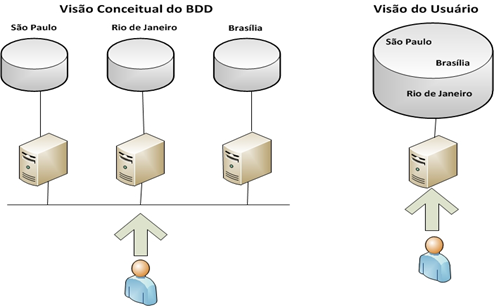
\includegraphics[height=7cm]{sistema_distribuido1.png}
\end{frame}
\subsection{Conhecendo o Hadoop}


\begin{frame}{Hadoop: Processamento Distribuído de Grandes Volumes de Dados}
    
\includegraphics[height=2cm]{hadoop.jpg}

\begin{block}{O que é}
Hadoop é um framework de computação distribuída projetado para armazenar e processar
grandes volumes de dados em clusters de computadores comuns (commodity hardware),
garantindo escalabilidade horizontal e tolerância a falhas.
\end{block}

\begin{block}{Ideia principal}
Ao invés de usar um supercomputador, o Hadoop divide o problema em várias partes
menores e executa cada parte em diferentes máquinas ao mesmo tempo.
Se uma máquina falhar, outra assume automaticamente sua função.
\end{block}


\end{frame}

\begin{frame}{Hadoop: Processamento Distribuído de Grandes Volumes de Dados}

\begin{block}{Componentes fundamentais}
\begin{itemize}
\item HDFS — sistema de arquivos distribuído e replicado
\item MapReduce — modelo de processamento paralelo
\item YARN — gerenciador de recursos do cluster
\end{itemize}
\end{block}

\end{frame}
\subsection{Hadoop File System (HDFS)}

\begin{frame}[fragile]{Acessando o Terminal do HDFS}
 
\begin{block}{Como funciona}
O Hadoop não possui um terminal próprio.
Utilizamos o terminal Linux (bash) e executamos comandos através do cliente HDFS:
\texttt{hdfs dfs}
\end{block}

\begin{block}{Primeiro comando}
\begin{verbatim}
hdfs dfs -ls /
\end{verbatim}
Se o comando listar diretórios, o sistema de arquivos distribuído
já está acessível.
\end{block}

\begin{block}{Interpretação}
A partir desse ponto, todos os comandos executados com
\texttt{hdfs dfs} manipulam arquivos armazenados no cluster,
não no computador local.
\end{block}

\end{frame}
\begin{frame}[fragile]{Operações Básicas no HDFS}

\begin{verbatim}
hdfs dfs -ls /
\end{verbatim}
\begin{verbatim}
hdfs dfs -mkdir /dados

\begin{verbatim}
hdfs dfs -put arquivo.txt /dados
\end{verbatim}

\begin{verbatim}
hdfs dfs -cat /dados/arquivo.txt
\end{verbatim}

\begin{verbatim}
hdfs dfs -get /dados/arquivo.txt
\end{verbatim}

\end{frame}
\begin{frame}{Comparação: Linux vs HDFS}

\begin{block}{Equivalência de comandos}

\begin{center}
\begin{tabular}{c|c}
Linux & HDFS \\ \hline
ls & hdfs dfs -ls \\
mkdir & hdfs dfs -mkdir \\
cp & hdfs dfs -put / -get \\
cat & hdfs dfs -cat
\end{tabular}
\end{center}

\end{block}

\begin{block}{Importante}
Os comandos parecem Linux, mas operam em máquinas do cluster.
Os dados não estão no computador local.
\end{block}

\begin{block}{Conclusão}
O HDFS funciona como um sistema de arquivos remoto acessado
via terminal.
\end{block}

\end{frame}
\subsection{Redundância no Hadoop}

\begin{frame}{Redundância no Hadoop}
\begin{block}{Ideia central}
O Hadoop foi projetado assumindo que falhas de hardware são normais.
Em vez de evitar falhas, o sistema tolera falhas automaticamente.
\end{block}

\begin{itemize}
    \item Usa armazenamento distribuído (HDFS)
    \item Dados são replicados entre máquinas
    \item O sistema continua funcionando mesmo com nós quebrados
\end{itemize}
\end{frame}
\begin{frame}{Exemplo de Replicação}

\begin{table}[]
\centering
\begin{tabular}{c|c|c|c}
Bloco & Nó A & Nó B & Nó C \\ \hline
B1 & cópia & cópia & cópia \\
B2 & cópia & cópia & cópia \\
B3 & cópia & cópia & cópia
\end{tabular}
\end{table}

\begin{block}{Resultado}
Se um computador falhar, os dados continuam acessíveis nos outros.
\end{block}
\end{frame}


\subsection{Ecossistema Hadoop}

\begin{frame}{Ecossistema Hadoop}
  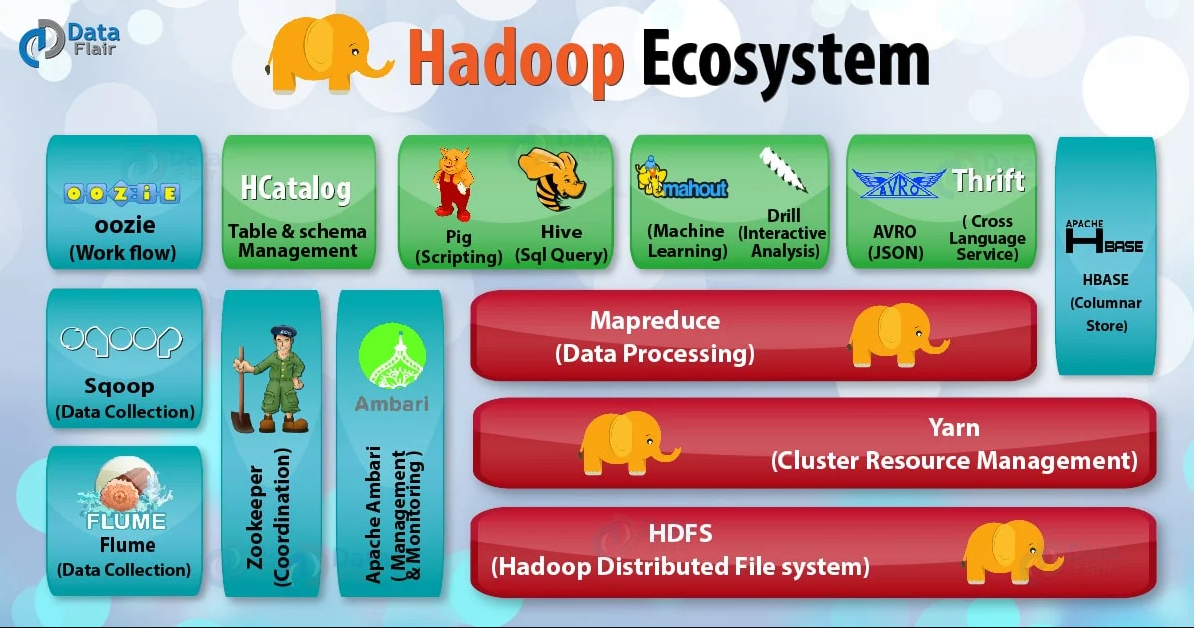
\includegraphics[height=6.5cm]{hadoop_zologico.png}
\end{frame}

\subsection{Sistemas de Proteção}

\begin{frame}{Sistema de Proteção — Conceito}
\small
Um \textbf{sistema de proteção} é um sistema especializado associado a outro sistema principal.

\begin{itemize}
    \item Atua como supervisor independente;
    \item Observa o ambiente e o comportamento do sistema controlado;
    \item Intervém quando o sistema principal não reage corretamente.
\end{itemize}

\begin{block}{Aplicações típicas}
\begin{itemize}
    \item Controle industrial (plantas químicas)
    \item Equipamentos críticos
    \item Trens autônomos
\end{itemize}
\end{block}

\end{frame}
\begin{frame}{Exemplo: Trem Autônomo}
\small

\textbf{Situação:} o trem ultrapassa sinal vermelho.

\begin{enumerate}
    \item O sistema principal deveria desacelerar
    \item Se isso não ocorrer
    \item O sistema de proteção assume o controle
    \item Freios são acionados automaticamente
\end{enumerate}

\begin{alertblock}{Importante}
O sistema de proteção não depende da decisão do sistema principal.
Ele atua mesmo se o software de controle estiver defeituoso.
\end{alertblock}

\end{frame}
\begin{frame}{Visão esquemática de um sistema de proteção}
  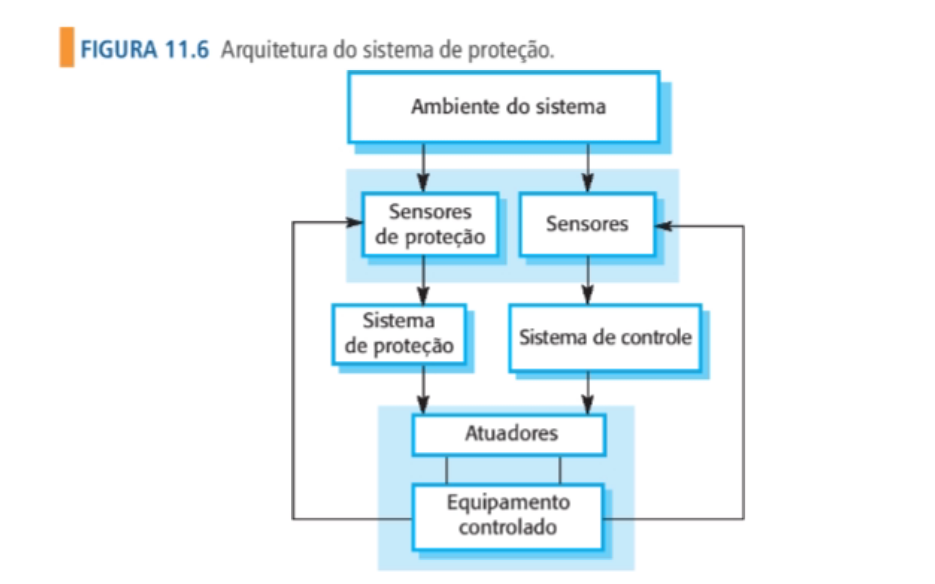
\includegraphics[height=6.5cm]{sistemas_protecao.png}
\end{frame}
\begin{frame}{Funcionamento do Sistema de Proteção}
\small

O sistema monitora dois elementos:

\begin{itemize}
    \item O comportamento do sistema controlado
    \item O ambiente físico ao redor
\end{itemize}

\begin{block}{Ação de Proteção}
Se for detectada uma situação perigosa:
\begin{itemize}
    \item O processo é desligado
    \item Ou mecanismos de segurança são acionados
\end{itemize}
Exemplo: abertura de válvula de alívio de pressão
\end{block}

\end{frame}
\begin{frame}{Sensores e Redundância}
\small

Arquiteturas de proteção utilizam redundância física:

\begin{itemize}
    \item Dois conjuntos de sensores
    \begin{itemize}
        \item Sensores de operação normal
        \item Sensores dedicados à segurança
    \end{itemize}

    \item Sensores de backup em caso de falha
    \item Atuadores redundantes
\end{itemize}

\begin{block}{Motivação}
O sistema de proteção deve continuar operando
mesmo se o próprio sistema monitorado estiver falhando.
\end{block}

\end{frame}
\begin{frame}{Ideia Central dos Sistemas de Proteção}
\centering
\vspace{0.5cm}

\Large
O sistema principal tenta operar corretamente

\vspace{0.4cm}

\Large
O sistema de proteção garante que nada catastrófico aconteça

\vspace{0.8cm}

\small
Ele não evita defeitos — ele evita acidentes.
\end{frame}
\begin{frame}{Função Essencial do Sistema de Proteção}
\small

Um sistema de proteção implementa apenas a funcionalidade crítica
necessária para mover o sistema de um estado perigoso para um estado seguro.

\begin{itemize}
    \item Não executa operação normal
    \item Atua somente em emergência
    \item Pode desligar completamente o sistema
\end{itemize}

\begin{block}{Arquitetura Geral}
Sistema principal complexo + sistema de backup simples e independente
\end{block}

\end{frame}
\begin{frame}{Exemplo: Sistema de Backup do Ônibus Espacial}
\small

O software de controle do ônibus espacial possuía um sistema secundário
com funcionalidade limitada:

\begin{itemize}
    \item Não realizava todas as operações de navegação
    \item Não executava todas as rotinas de controle
    \item Apenas a função essencial: \textbf{"levá-lo para casa"}
\end{itemize}

\begin{alertblock}{Objetivo}
Caso o sistema principal falhasse, o sistema de proteção conseguiria
realizar o pouso com segurança.
\end{alertblock}

\end{frame}
\begin{frame}{Confiabilidade do Sistema de Proteção}
\small

Como o sistema é pequeno e simples:

\begin{itemize}
    \item É possível validar melhor a especificação
    \item Verificar formalmente o comportamento
    \item Investir mais na prevenção e detecção de defeitos
\end{itemize}

\begin{block}{Meta de Engenharia}
Probabilidade muito baixa de falha sob demanda:

\[
P(falha \mid demanda) \approx 0{,}001
\]

Demandas são raras $\Rightarrow$ falhas extremamente raras
\end{block}

\end{frame}
\subsection{Detecção de falhas no Hadoop}

\begin{frame}{Detecção de Falhas  no hadoop}
    
\includegraphics[height=2cm]{hadoop.jpg}

\begin{block}{Heartbeat}
Cada máquina envia sinais periódicos ao servidor principal.
\end{block}

Se parar de responder:
\begin{enumerate}
    \item O sistema detecta falha
    \item Identifica blocos perdidos
    \item Cria novas cópias automaticamente
\end{enumerate}

\begin{alertblock}{Importante}
O cluster se auto-repara sem intervenção humana.
\end{alertblock}
\end{frame}
\begin{frame}{Arquitetura de nós hadoop}
  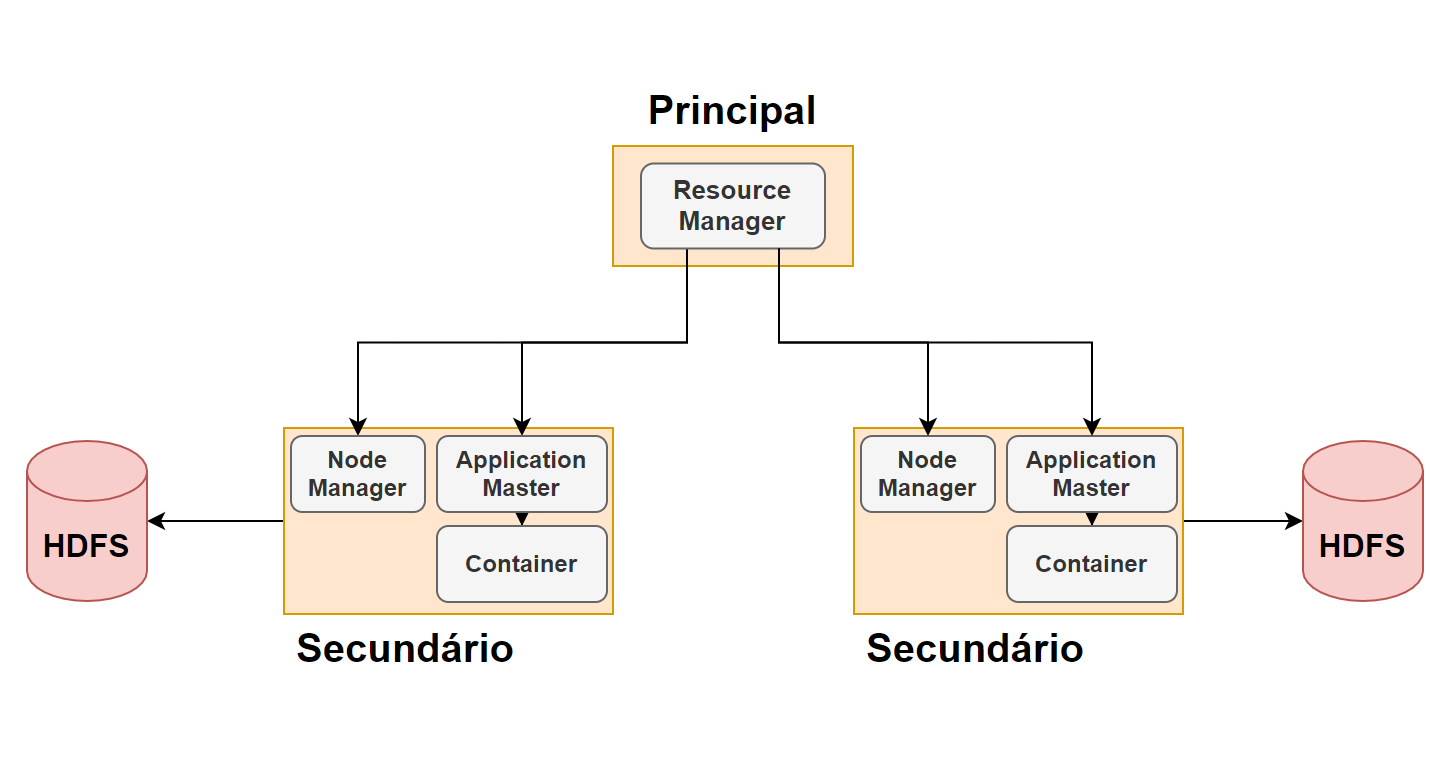
\includegraphics[height=6.5cm]{hadoop_2.png}
\end{frame}



\subsection{Arquitetura de Automonitoramento}

\begin{frame}{Arquitetura de Automonitoramento — Conceito}
\small

O próprio sistema monitora sua operação e detecta falhas internas.

\begin{itemize}
    \item Cálculos executados em canais independentes
    \item Resultados são comparados
    \item Divergência indica defeito
\end{itemize}

\begin{block}{Princípio}
Se dois sistemas iguais recebem a mesma entrada,
devem produzir a mesma saída.
\end{block}

\end{frame}
\begin{frame}{Detecção de Falhas}
\small

Processo de funcionamento:

\begin{enumerate}
    \item Entrada é enviada para múltiplos canais
    \item Cada canal calcula independentemente
    \item Resultados são comparados
\end{enumerate}

\begin{alertblock}{Resultado}
\begin{itemize}
    \item Iguais → operação considerada correta
    \item Diferentes → falha detectada
\end{itemize}
\end{alertblock}

O sistema então sinaliza erro e transfere o controle.

\end{frame}
\subsection{Diversidade de Hardware}

\begin{frame}{Diversidade de Hardware}
\small

Para evitar falhas comuns, os canais não devem ser idênticos.

\begin{itemize}
    \item Processadores diferentes
    \item Chipsets de fabricantes distintos
    \item Implementações físicas independentes
\end{itemize}

\begin{block}{Motivação}
Reduzir a probabilidade de defeitos de projeto afetarem todos os canais ao mesmo tempo.
\end{block}

\end{frame}
\subsection{Diversidade de Software}

\begin{frame}{Diversidade de Software}
\small

Também é necessário evitar falhas simultâneas de software.

\begin{itemize}
    \item Implementações independentes
    \item Equipes diferentes
    \item Linguagens de programação diferentes
\end{itemize}

\begin{alertblock}{Problema evitado}
O mesmo bug não deve existir em todos os canais.
\end{alertblock}

\end{frame}
\begin{frame}{Nó master e slave no hadoop}
  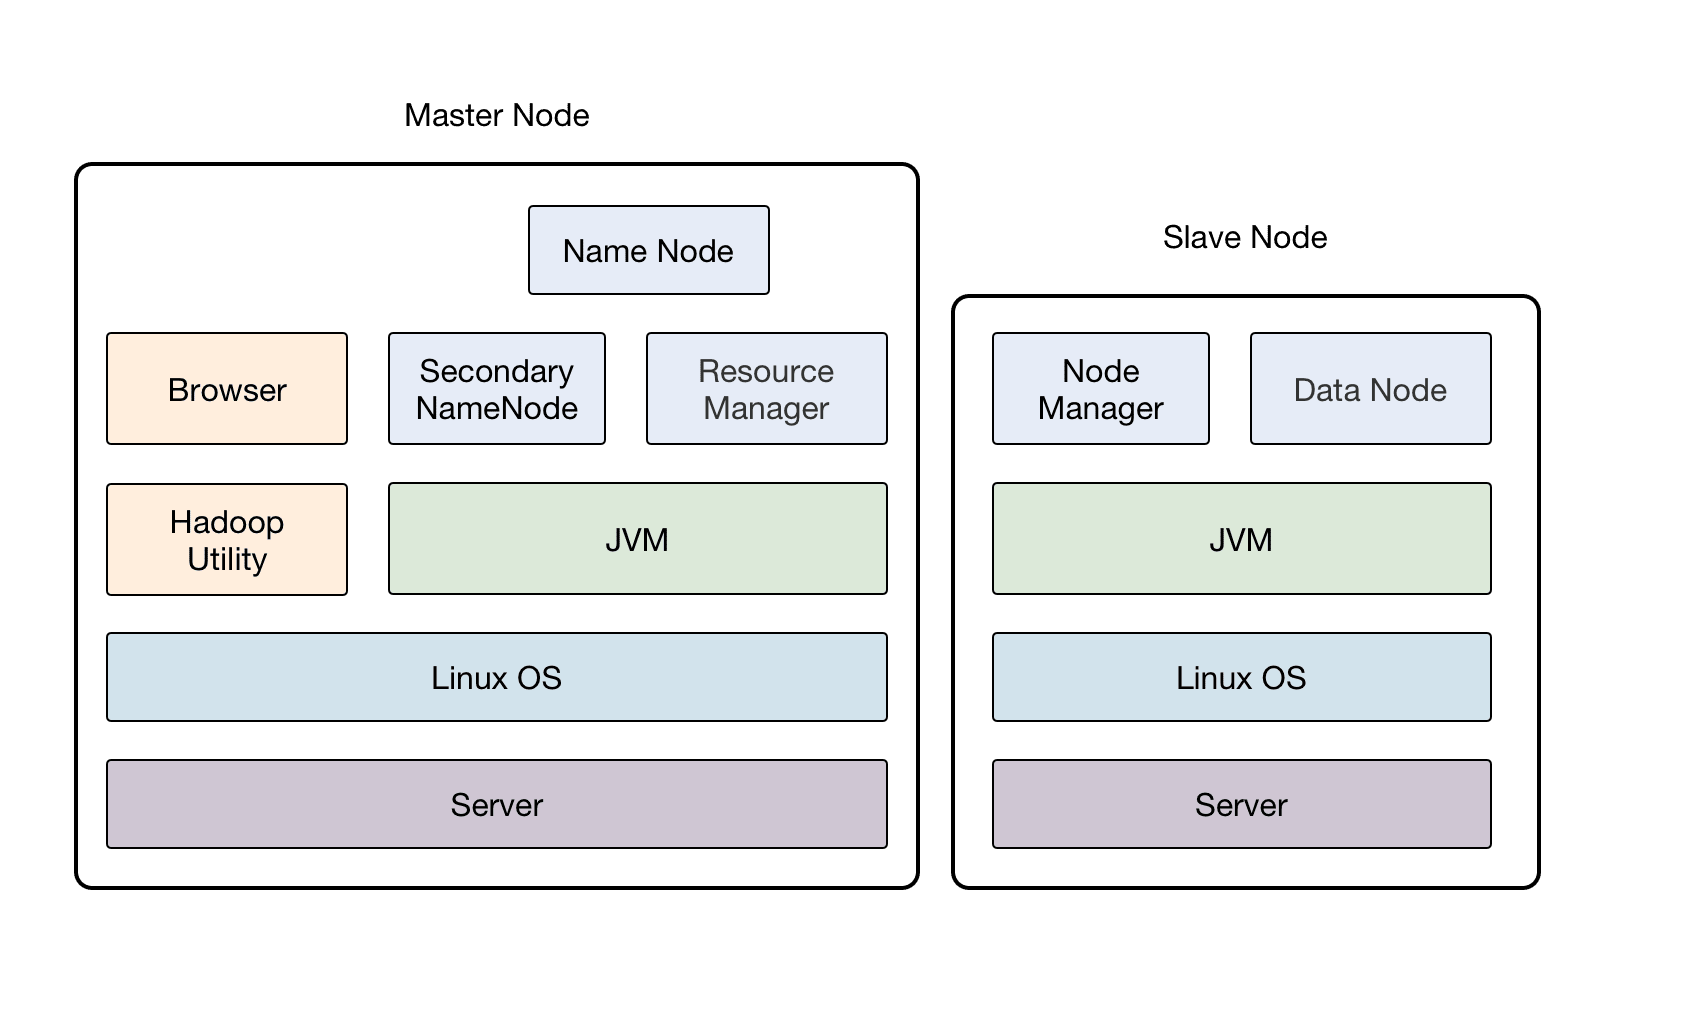
\includegraphics[height=7.5cm]{hadoop3.png}
\end{frame} 

\begin{frame}{Confiabilidade vs Disponibilidade}
\small

A arquitetura pode ser usada quando a confiabilidade é mais importante que disponibilidade.

\begin{itemize}
    \item Se houver divergência → sistema desliga
\end{itemize}

\begin{block}{Exemplo}
Sistemas médicos de diagnóstico:
uma resposta errada é pior que parar o sistema.
\end{block}

\end{frame}
\begin{frame}{Alta Disponibilidade}
\small

Quando o sistema não pode parar:

\begin{itemize}
    \item Vários sistemas automonitorados em paralelo
    \item Unidade de chaveamento seleciona saída válida
\end{itemize}

\begin{block}{Objetivo}
Manter operação mesmo com falhas internas.
\end{block}

\end{frame}
\begin{frame}{Exemplo: Controle de Voo}
\small

Sistema de controle de voo usa múltiplos computadores:

\begin{itemize}
    \item Computações paralelas com mesma entrada
    \item Filtros detectam saída defeituosa
    \item Saída alternativa é selecionada
\end{itemize}

O sistema pode continuar operando mesmo com múltiplas falhas.

\end{frame}
\begin{frame}{Estratégias de Diversidade}
\small

Diversidade aplicada de várias formas:

\begin{enumerate}
    \item Processadores diferentes
    \item Fornecedores distintos
    \item Software secundário mais simples
    \item Equipes independentes
    \item Linguagens de programação diferentes
\end{enumerate}

\end{frame}
\begin{frame}{Ideia Central do Automonitoramento}
\centering

\Large
O sistema não tenta evitar falhas

\vspace{0.4cm}

\Large
Ele detecta falhas imediatamente

\vspace{0.8cm}

\small
A segurança vem da comparação entre múltiplas computações independentes.

\end{frame}
\subsection{Programação N-versões}

\begin{frame}{Programação N-versões}
\small

A programação N-versões é uma técnica de tolerância a defeitos baseada
em redundância de software.

\begin{itemize}
    \item Várias implementações independentes do mesmo sistema
    \item Executadas em paralelo
    \item Resultados comparados por votação
\end{itemize}

\begin{block}{Objetivo}
Garantir saída correta mesmo se uma versão falhar.
\end{block}

\end{frame}
\begin{frame}{Origem: Redundância Modular Tripla}
\small

A ideia foi inspirada na tolerância a falhas de hardware:

\begin{itemize}
    \item Triple Modular Redundancy (TMR)
    \item Três unidades executam o mesmo cálculo
    \item Um votador escolhe o resultado majoritário
\end{itemize}

\begin{alertblock}{Comportamento}
Se uma unidade falhar, sua saída é ignorada.
\end{alertblock}

\end{frame}
\begin{frame}{Sistema de Votação}
\small

O comparador recebe múltiplas saídas:

\[
saida = maioria(saida_1, saida_2, saida_3)
\]

\begin{itemize}
    \item 2 iguais → resultado aceito
    \item 1 diferente → considerado defeituoso
\end{itemize}

\begin{block}{Reconfiguração}
O sistema pode remover automaticamente a unidade defeituosa
e continuar operando.
\end{block}

\end{frame}
\begin{frame}{Hipótese Fundamental}
\small

A técnica assume:

\begin{itemize}
    \item Falhas ocorrem independentemente
    \item Diferentes implementações não possuem o mesmo erro
\end{itemize}

\begin{alertblock}{Falha de modo comum}
Se todas as versões tiverem o mesmo defeito,
o sistema produzirá uma resposta errada consistente.
\end{alertblock}

\end{frame}
\begin{frame}{N-versões em Software}
\small

Extensão do conceito de TMR para software:

\begin{itemize}
    \item N implementações independentes
    \item Desenvolvidas por equipes diferentes
    \item Linguagens e algoritmos diferentes
\end{itemize}

Saídas incoerentes ou atrasadas são descartadas.

\end{frame}
\begin{frame}{Número de Versões}
\small

Para tolerar uma falha:

\[
N \ge 3
\]

\begin{itemize}
    \item Uma versão pode falhar
    \item Duas restantes definem o resultado correto
\end{itemize}

\begin{block}{Condição}
Pelo menos duas respostas coerentes devem existir.
\end{block}

\end{frame}
\begin{frame}{Aplicações}
\small

Utilizado em sistemas críticos de segurança:

\begin{itemize}
    \item Sinalização ferroviária
    \item Controle aeronáutico
    \item Proteção de reatores nucleares
\end{itemize}

A falha do sistema pode causar consequências catastróficas.

\end{frame}
\begin{frame}{Custos e Limitações}
\small

Vantagem:
\begin{itemize}
    \item Alta disponibilidade
\end{itemize}

Desvantagem:
\begin{itemize}
    \item Múltiplas equipes de desenvolvimento
    \item Alto custo de implementação
\end{itemize}

\begin{alertblock}{Uso típico}
Aplicado apenas quando não é possível depender
de um sistema de proteção simples.
\end{alertblock}

\end{frame}
\begin{frame}{Ideia Central da Programação N-versões}
\centering

\Large
Não confiar em uma implementação

\vspace{0.4cm}

\Large
Confiar no consenso entre implementações independentes

\vspace{0.8cm}

\small
A segurança vem da diversidade.

\end{frame}

\begin{frame}{Conceito}
Todas as arquiteturas tolerantes a defeitos dependem da diversidade de software.

\bigskip

Baseia-se no pressuposto de que implementações diferentes da mesma especificação:

\begin{itemize}
\item São independentes
\item Não possuem erros em comum
\item Não falham simultaneamente
\end{itemize}

\bigskip

Objetivo: aumentar a confiabilidade do sistema.
\end{frame}

%------------------------------------------------

\begin{frame}{Independência entre Times}
O software deve ser desenvolvido por times distintos:

\begin{itemize}
\item Sem comunicação entre si
\item Interpretações independentes da especificação
\item Redução de erros comuns
\end{itemize}

Isso reduz mal-entendidos coletivos da especificação.
\end{frame}

%------------------------------------------------

\begin{frame}{Políticas de Diversidade}
A organização pode exigir diferenças explícitas entre versões.

\begin{enumerate}
\item Diferentes métodos de projeto
\item Diferentes linguagens de programação
\item Diferentes ferramentas de desenvolvimento
\item Diferentes algoritmos
\end{enumerate}
\end{frame}

%------------------------------------------------

\begin{frame}{Exemplos de Diversidade}
\textbf{Métodos de projeto}
\begin{itemize}
\item Orientado a Objetos
\item Orientado a Funções
\end{itemize}

\textbf{Linguagens}
\begin{itemize}
\item Ada
\item C++
\item Java
\end{itemize}

\textbf{Ferramentas}
\begin{itemize}
\item Compiladores distintos
\item IDEs diferentes
\end{itemize}
\end{frame}

%------------------------------------------------

\begin{frame}{Diversidade de Algoritmos}
Pode-se exigir algoritmos diferentes para o mesmo problema.

\bigskip

Vantagem:
\begin{itemize}
\item Redução de falhas simultâneas
\end{itemize}

Desvantagem:
\begin{itemize}
\item Dificuldade em cumprir requisitos de desempenho
\item Restrição à liberdade de projeto
\end{itemize}
\end{frame}

%------------------------------------------------

\begin{frame}{Confiabilidade Teórica}
Se versões forem independentes:

\[
Confiabilidade_{global} = Confiabilidade_1 \times Confiabilidade_2 \times Confiabilidade_3
\]

Exemplo:

POFOD de cada canal = 0,001

Sistema com três canais:

\[
0,001^3 = 0,000000001
\]

Sistema torna-se um milhão de vezes mais confiável.
\end{frame}

%------------------------------------------------

\begin{frame}{Problema Prático}
Independência completa não ocorre na prática.

Estudos mostram que equipes independentes:

\begin{itemize}
\item Cometem erros semelhantes
\item Interpretam errado as mesmas partes da especificação
\end{itemize}
\end{frame}

%------------------------------------------------

\begin{frame}{Causas de Erros Comuns}
\begin{enumerate}
\item Mesma formação acadêmica
\item Mesmos livros e técnicas aprendidas
\item Dificuldade comum com especialistas do domínio
\end{enumerate}
\end{frame}

%------------------------------------------------

\begin{frame}{Erros de Requisitos}
Se os requisitos estiverem errados:

\begin{itemize}
\item Todas as versões estarão erradas
\end{itemize}

Se a especificação for ambígua:

\begin{itemize}
\item Todos podem interpretar da mesma forma equivocada
\end{itemize}
\end{frame}

%------------------------------------------------

\begin{frame}{Redução de Erros de Especificação}
Criar especificações independentes em formatos diferentes:

\begin{itemize}
\item Especificação formal
\item Modelo baseado em estados
\item Linguagem natural
\end{itemize}

\bigskip

Limitação: não resolve erros de requisitos.
\end{frame}

%------------------------------------------------

\begin{frame}{Resultados Experimentais}
Estudos mostram:

Sistema de três canais é de 5 a 9 vezes mais confiável que sistema único.

\bigskip

Abordagens N-versões geralmente aumentam a confiabilidade.
\end{frame}

%------------------------------------------------

\begin{frame}{Custo vs Benefício}
Nem sempre compensa:

\begin{itemize}
\item Alto custo de desenvolvimento
\item Sistema único bem projetado pode ser suficiente
\end{itemize}

Recomendado principalmente para:

\begin{itemize}
\item Sistemas críticos de segurança
\item Sistemas de missão
\end{itemize}
\end{frame}

%------------------------------------------------

\begin{frame}{Alternativa Prática}
Pode ser suficiente:

\begin{itemize}
\item Sistema principal
\item Backup simples com funções limitadas
\end{itemize}

Até o sistema principal ser reiniciado.
\end{frame}

%------------------------------------------------
\section{Conclusão}

\begin{frame}{Conclusão}
Diversidade de software:

\begin{itemize}
\item Aumenta confiabilidade
\item Não garante independência total
\item Possui alto custo
\item Indicado para sistemas críticos
\end{itemize}
\end{frame}
\end{document}
